%***********************************************************************
% PLEASE LEAVE THIS PART UNCHANGED
% No problem!
%***********************************************************************

\documentclass[twoside]{report}
\usepackage{iwsm}
\usepackage{graphicx}
\usepackage{amsmath, amssymb}
\usepackage{booktabs}

\begin{document}

%***********************************************************************
% PLEASE INSERT YOUR CONTENT FROM HERE
%***********************************************************************

% Title and running title to be used as left header:
\title{Graphical Assessment of Probabilistic Precipitation Forecasts}
\titlerunning{Graphical Assessment of Probabilistic Forecasts}

% Authors and running list of authors to be used as right header:
\author{Reto Stauffer\inst{1}\,\inst{2}, Moritz N. Lang\inst{1}, Achim Zeileis\inst{1}}
\authorrunning{Stauffer et\,al.}

% Institutes of all authors
% Include city and country of each institute, do not include the full address.
\institute{Department of Statistics, Universit\"at Innsbruck, Austria
\and Digital Science Center, Universit\"at Innsbruck, Austria}

% E-mail of presenting author for correspondence
\email{Reto.Stauffer@uibk.ac.at}

% Brief abstract of the paper:
\abstract{
    Accurate and reliable probabilistic predictions have been becoming more and more
    important over the last decades and they are an essential
    tool for proper risk assessment and strategic planning.
    In order to provide full probabilistic forecasts, distributional regression
    models are frequently used.  Such models range from basic generalized
    linear models (GLM) over generalized additive models (GAM) to generalized
    additive models for locate, scale, and shape (GAMLSS) and other types of
    refined distributional regression models.

    For assessing the goodness of fit of such probabilistic regression models,
    graphical assessment techniques are an important complement to proper
    scoring rules and help to identify possible model misspecifications.
    Based on a case study of probabilistic precipitation forecasts, three
    different model specifications are evaluated graphically to reveal
    different sources of misspecification such as censoring at zero,
    hereoscedasticity, and heavy tails. The graphics either evaluate
    marginal calibration by comparing observed and fitted frequencies
    using variations of so-called rootograms. Or alternatively
    they assess probabilistic calibration by evaluating the distribution of the
    probability integral transform (PIT) on different scales using histograms or
    variations of quantile-quantile plots. Relative strengths and
    weaknesses in revealing the sources of misfit are highlighted.
    
    A unified implementation is provided in the newly developed \emph{R}~package \emph{topmodels}
    (\texttt{https://topmodels.R-Forge.R-project.org/}).

}

% Keywords (at most 5):
\keywords{Graphical model assessment; Distributional regression}

% Produce the title:
\maketitle

%***********************************************************************

% Sections and subsections (do not use lower levels):

\section{Case study}

Weather forecasts are typically generated by physically-based numerical weather
prediction models. To account for uncertainty, multiple forecasts are created
with slightly modified conditions which build an ensemble.
This allows to not only retrieve information about the expected amount of precipitation
but also the associated uncertainty. To better calibrate these raw ensemble
forecasts, statistical post-processing is typically applied.

Revisiting three model specifications considered by Messner, Mayr, and Zeileis (2010),
we use different graphical model assessment techniques for identifying possible
model misspecifications and thus aiding the selection of a well-calibrated
model.

% \subsection{Data}

The data used contains observed accumulated precipitation amounts for
Innsbruck and the corresponding ensemble mean ($\text{ensmean}$) and
ensemble standard deviation ($\text{enssd}$) of total accumulated precipitation amounts
between $5$ and $8$ days in advance.
Following previous studies, the square root of precipitation is used which has
been shown to improve the calibration.

% \subsection{Statistical models}

For comparison, three models are employed. A homoscedastic Gaussian linear regression
model which does not properly account for the non-negative nature of precipitation,
and two heteroscedastic regression models, left-censored at zero --
one assuming a Gaussian and one a logistic underlying response distribution.

\begin{table}[!ht]\centering
    \begin{tabular}{lll}
         Distribution                              & Location                                         & Scale \\
        \midrule[0.09 em]
        $y_i \sim \mathcal{N}(\mu_i, \sigma_i^2)$   & $\hat{\mu}_i = \hat{\beta}_0 + \hat{\beta}_1 \cdot \text{ensmean}_i$ & $\log(\hat{\sigma}_i) = \hat{\gamma}_0$ \\
        $y_i \sim \mathcal{N}_0(\mu_i, \sigma_i^2)$ & $\hat{\mu}_i = \hat{\beta}_0 + \hat{\beta}_1 \cdot \text{ensmean}_i$ & $\log(\hat{\sigma}_i) = \hat{\gamma}_0 + \hat{\gamma}_1 \cdot \log(\text{enssd}_i)$ \\
        $y_i \sim \mathcal{L}_0(\mu_i, \sigma_i^2)$ & $\hat{\mu}_i = \hat{\beta}_0 + \hat{\beta}_1 \cdot \text{ensmean}_i$ & $\log(\hat{\sigma}_i) = \hat{\gamma}_0 + \hat{\gamma}_1 \cdot \log(\text{enssd}_i)$ \\
        \bottomrule[0.09 em]
    \end{tabular}
\end{table}


\section{Model assessment}

According to the seminal work of Gneiting, Balabdaoui, and Raftery (2007),
probabilistic forecasts aim to maximize the sharpness of the predictive
distributions subject to calibration. Moreover, this can be further
distinguished into marginal and probabilistic calibration.

\subsection{Marginal calibration}

Marginal calibration is generally concerned with whether the observed
frequencies of the response variable $y_i$ match the corresponding expected
frequencies from the model.  For continuous response variables, frequencies
for intervals $(b_j, b_{j + 1}]$ are considered based on breaks $b_j$
($j = 1, \dots, k$). The expected frequencies are computed based on the
predicted cumulative distribution function (CDF) $F(\cdot | \hat \theta)$
where $\theta = (\mu, \sigma)$ denotes the joint model parameters.

$$
\text{observed}_j = \sum_{i=1}^N I(y_i \in (b_j, b_{j+1}]),
$$

$$
\text{expected}_j = \sum_{i=1}^N \big[ F(b_{j+1} | \hat{\theta}_i) - F(b_{j} | \hat{\theta}_i) \big].
$$

Figure~\ref{stauffer:fig1} shows hanging rootograms for the two Gaussian
models, where the observed frequencies are hanging from the expected ones. The
marginal calibration is assessed on the observational scale, which allows a
direct interpretation.  The heteroscedastic Gaussian model clearly underfits
zero precipitation amounts as it is not accounting for the observed point mass
at zero. Additionally, a weak wavelike pattern indicates a slight overfitting
of precipitation sums between $0$ and $5$ and an underfitting of precipitation
above. In contrast, the heteroscedastic left-censored Gaussian model provides a
fairly good marginal fit.

However, due to the aggregation over all individual predictive CDFs
$F(y_i|\hat{\theta}_i)$ for $i = 1, \dots, N$, a statement about a
possible violation of the distributional assumption is not easily possible.

\begin{figure}[!ht]\centering
    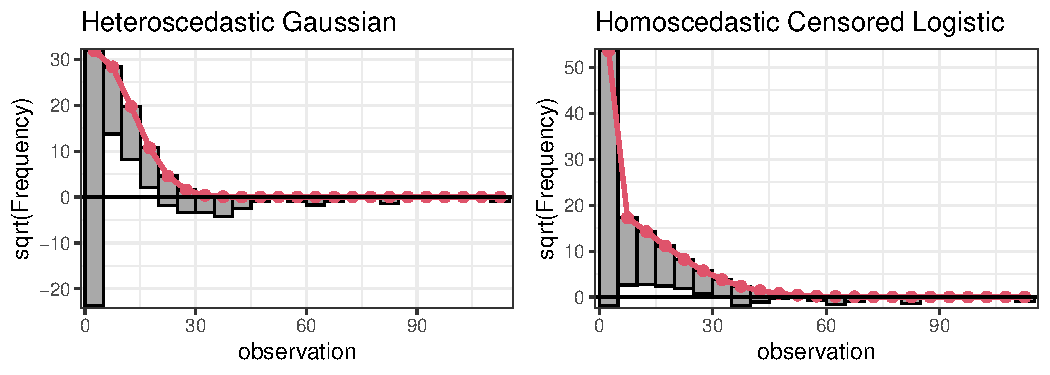
\includegraphics[width=\textwidth]{Stauffer-rootograms}
    \caption{\label{stauffer:fig1}
        Hanging rootograms for the homoscedastic Gaussian model (left)
        and the heteroscedastic left-censored Gaussian model (right).
        Expected frequencies shown in red (line), observed frequencies
        in gray (bars).
    }
\end{figure}

\subsection{Probabilistic calibration}

Compared to the marginal calibration which is obtained on the observation
scale, the probabilistic calibration is always performed on the probability
scale by considering the probability integral transform (PIT) $u_i = F(y_i | \hat{\theta}_i)$.
Additionally, this may need to be randomized for (partially) discrete observations
to obtain uniformly distributed PIT values if the model is well calibrated.
Alternatively, the PIT values can be mapped to other scales, e.g.,
by using the inverse of a standard normal CDF $\Phi(\cdot)$, 
to obtain (randomized) quantile residuals ($r_i$) as suggested by Dunn and Smyth (1996).

$$
r_i = \Phi^{-1}\big(u_i)~~\text{with}~~u_i = \begin{cases}
    F(y_i | \hat{\theta}_i) & \text{if}~F(\cdot)~\text{continuous}  \\
    U\big[F(y_i - 1 | \hat{\theta}_i), F(y_i | \hat{\theta}_i)\big] & \text{if}~F(\cdot)~\text{discrete}
\end{cases}
$$

Whether the distribution of $u_i$ or $r_i$ is uniform or normal, respectively,
can then be checked using standard graphics like histograms or quantile-quantile
(Q-Q) plots. As small too medium deviations can be quite hard
to detect in Q-Q plots, detrending the plot by considering deviations of empirical
and theoretical quantiles (also called worm plots) can be helpful.

\begin{figure}[!ht]\centering
    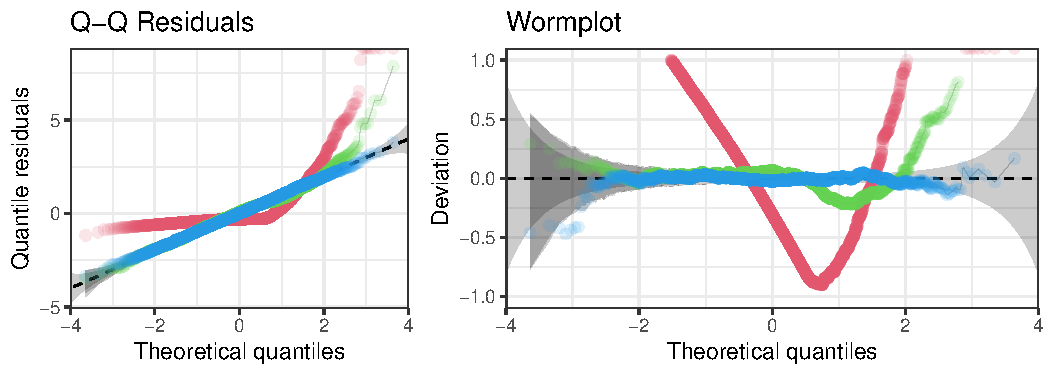
\includegraphics[width=\textwidth]{Stauffer-qqresiduals}
    \caption{\label{stauffer:fig2} 
        Q-Q plot (left) and worm plot (right) for the homoscedastic
        Gaussian model (red), as well as the heteroscedastic left-censored
        Gaussian (green) and the heteroscedastic left-censored logistic (blue) model.
    }
\end{figure}

Both, the Q-Q plot and the worm plot included in Figure\,\ref{stauffer:fig2}
show an obvious misfit of the homoscedastic Gaussian model on both tails of the
distribution. While the marginal calibration (Fig.\,\ref{stauffer:fig1})
clearly shows that this is mainly due to missing censoring, the probabilistic
calibration in this example does not allow to uncover the sources causing this
lack of fit.

While the scale itself is not easily interpretable, the probabilistic calibration
allows to check if the distributional assumption is correct.  Comparing both
left-censored heteroscedastic models, a slight advantage can be seen for the
one using a left-censored logistic distribution as its heavier tails lead to a
better fit, especially for high quantiles.

%***********************************************************************

% References should be placed in the text in author (year) form.
% The list of references should be placed below IN ALPHABETICAL ORDER.
% (Please follow the format of the examples very tightly).

\references
\begin{description}
% QQ REsiduals
    \item [Dunn, P.K., and Smyth G.K.] (1996).
        Randomized Quantile Residuals.
        {\it Journal of Computational and Graphical Statistics},
        {\bf 5}(3), 236\,--\,244.
% Reliability diagram
%\item [Bröcker, J., and Smith, L.A.] (2007).
%    Increasing the Reliability of Reliability Diagrams.
%    {\it Weather and Forecasting},
%    {\bf 22}(3), 651\,--\,61.
% Ensemble forecasting
%\item[Gneiting, T., and Raftery, A.E.] (2005).
%    Weather Forecasting with Ensemble Methods.
%    {\it Science},
%    {\bf 310}(5746), 248\,--\,249.
% Proper scoring rules (CRPS)
%\item[Gneiting, T., and Raftery, A.E.] (2007).
%    Strictly Proper Scoring Rules, Prediction, and Estimation.
%    {\it ournal of the American Statistical Association},
%    {\bf 102}(477), 359\,--\,78.
% Maximize sharpness subject to calibration
\item[Gneiting, T., Balabdaoui, F., and Raftery, A.E.] (2007).
    Probabilistic Forecasts, Calibration and Sharpness.
    {\it Journal of the Royal Statistical Society: Series B (Methodological)},
    {\bf 69}(2), 243\,--\,268.
% Rootograms (marginal calibration)
%\item [Kleiber, C., and Zeileis A.] (2016).
%    Visualizing Count Data Regressions Using Rootograms.
%    {\it The American Statistician},
%    {\bf 70}(3), 296\,--\,303.
% Rain stuff 
\item [Messner, J.W., Mayr, G.J., and Zeileis A.] (2016).
    Heteroscedastic Censored and Truncated Regression with crch.
    {\it The R Journal},
    {\bf 8}(1), 173\,--\,181.
% PIT residuals (specifically)
%\item [Warton, D.I., Thibaut, L., and Wang, Y.A.] (2017).
%    The Pit-Trap---{A} ``Model-Free'' Bootstrap Procedure for Inference About
%    Regression Models with Discrete, Multivariate Responses.
%    {\it PLOS ONE},
%    {\bf 12}(7), 1\,--\,18.
% Reliability diagram
%\item [Wilks, D.] (2011).
%    {\it Statistical Methods in the Atmospheric Sciences 3rd ed}.
%    Academic Press.
\end{description}

\end{document}
